\chapter{天空中的太阳：昼夜与季节}\label{ch:g3:sun-days-seasons}

六月里，晚饭后你还在金色阳光中外面玩耍；
十二月里，你还没放学到家，路灯就亮了。
太阳仍保持着它的老习惯——从一侧升起，越过头顶，再从另一侧落下——
但它在天空中走过的路线，并非全年都一样。
连续跟踪一整年，你就能发现\omterm{def:g3:sun-days-seasons:year}{季节}的变化。

\section{太阳变化的路线}

\begin{example}[夏天的路线，冬天的路线]\label{ex:g3:sun-days-seasons:roads}
观察仲夏时太阳的弧线：它升起得早，爬得很高，
正午时几乎到达头顶——落得也晚：这是一条又长又高的路线，
白天也很长。仲冬时，弧线又低又短：太阳升起得晚，
从不会升到屋顶以上很高，午后中段就落下了。
春天和秋天介于两者之间，路线居中，
昼与夜的\omterm{def:g2:measuring-time:duration}{时长}
几乎相等。
\end{example}

\begin{omfigure}
\begin{tikzpicture}[scale=0.85]
  \draw[thick] (0,0) -- (11,0);
  \draw[dashed, omThm, thick] (1.0,0.2) .. controls (3.5,4.6)
    and (7.5,4.6) .. (10.0,0.2);
  \fill[omThm] (5.5,3.5) circle (0.3);
  \node[above, font=\small, omThm] at (5.5,3.9) {仲夏：高而长};
  \draw[dashed, omDef, thick] (2.6,0.15) .. controls (4.4,1.7)
    and (6.6,1.7) .. (8.4,0.15);
  \fill[omDef] (5.5,1.3) circle (0.3);
  \node[above, font=\small, omDef] at (2.9,1.35) {仲冬：低而短};
\end{tikzpicture}

{\small 太阳在同一地平线上的两条极端路线。
夏季的高弧线需要很多\omterm{ex:g2:measuring-time:clock}{小时}才能走完；
冬季的低弧线在午后中段就走完了。}
\end{omfigure}

\begin{proposition}[正午规律]\label{prop:g3:sun-days-seasons:midday}
每个\omterm{def:g3:sun-days-seasons:year}{季节}里，太阳都在正午时分升得最高——
此时每个\omterm{def:g1:light-and-shadows:shadow}{影子}在当天最短，
并且与昨天、明天正午的\omterm{def:g1:light-and-shadows:shadow}{影子}指向同一方向。
正午的\omterm{def:g1:light-and-shadows:shadow}{影子}是大自然中最可靠的“箭头”。
\end{proposition}

\begin{example}[从影子读出季节]\label{ex:g3:sun-days-seasons:shadowlength}
正午\omterm{def:g1:light-and-shadows:shadow}{影子}的\emph{长度}随\omterm{def:g3:sun-days-seasons:year}{季节}而变化：夏天时，太阳几乎在头顶，
一根立杆的正午\omterm{def:g1:light-and-shadows:shadow}{影子}只是短短一截；
冬天时，太阳低低地挂着，同一根立杆投下很长的正午\omterm{def:g1:light-and-shadows:shadow}{影子}。
每月在地面上标出一次正午\omterm{def:g1:light-and-shadows:shadow}{影子}的顶端，
这些标记会在一年中来回移动，
就像一个缓慢的单摆。
\end{example}

\section{影子钟}

\begin{definition}[日晷]\label{def:g3:sun-days-seasons:sundial}
\emph{日晷}\index{日晷}是一种由\omterm{def:g1:light-and-shadows:shadow}{影子}组成的钟：一根立杆或一块薄板立在阳光下，
周围标有刻线，表示每个整点时\omterm{def:g1:light-and-shadows:shadow}{影子}落在何处。
太阳沿着它的弧线移动，\omterm{def:g1:light-and-shadows:shadow}{影子}
扫过刻线——缓慢、无声，
且没有任何活动的部件。
\end{definition}

\begin{method}[制作影子钟]\label{met:g3:sun-days-seasons:build}
在一个晴朗的早晨，选一个全天都有阳光的地方：
\begin{enumerate}
  \item 在平地上竖直插入一根直棍
        （也可以把它立在一桶沙子中）；
  \item 每隔一\omterm{ex:g2:measuring-time:clock}{小时}，正好整点时，用小石子标出\omterm{def:g1:light-and-shadows:shadow}{影子}的顶端，
        并用粉笔在石子上写下时刻。
  \item 一直记到傍晚。
\end{enumerate}
明天，\omterm{def:g1:light-and-shadows:shadow}{影子}会准时经过你的小石子，
你的这根棍子就能报时了。（至少在一段时间内能用——随着\omterm{def:g3:sun-days-seasons:year}{季节}变化，
\omterm{def:g1:light-and-shadows:shadow}{影子}也会慢慢移动，小石子会逐渐指向错误的时刻。）
\end{method}

\begin{omfigure}
\begin{tikzpicture}[scale=0.85]
  \draw[thick] (0.5,0) -- (10.5,0);
  \draw[very thick] (5.5,0) -- (5.5,1.7);
  \draw[line width=3pt, omExo] (5.5,0) -- (2.2,0.9);
  \draw[line width=3pt, omExo, opacity=0.6] (5.5,0) -- (4.1,1.35);
  \draw[line width=3pt, omExo, opacity=0.35] (5.5,0) -- (5.5,1.5);
  \draw[line width=3pt, omExo, opacity=0.6] (5.5,0) -- (6.9,1.35);
  \draw[line width=3pt, omExo] (5.5,0) -- (8.8,0.9);
  \node[font=\footnotesize] at (1.8,1.0) {早晨};
  \node[font=\footnotesize] at (5.5,1.9) {正午：最短};
  \node[font=\footnotesize] at (9.4,1.0) {傍晚};
\end{tikzpicture}

{\small 一根棍子，一天之内：\omterm{def:g1:light-and-shadows:shadow}{影子}像一只缓慢的指针扫过，
在一天的两端最长，正午时最短。}
\end{omfigure}

\section{一年与四季}

\begin{definition}[一年与四季]\label{def:g3:sun-days-seasons:year}
地球在每天自转的同时，还沿着一条巨大的轨道
\emph{绕太阳}运行——绕行一周需要一个
\emph{年}\index{年}，约 $365$ 天。沿着这一圈，太阳在我们天空中的路线
缓慢地升高又降低，我们经历
四个\emph{季节}\index{季节}：春、夏、秋、冬
——然后又是春天，一圈又一圈。
\end{definition}

\begin{example}[四季]\label{ex:g3:sun-days-seasons:quarters}
夏季：太阳高挂，白天长，正午\omterm{def:g1:light-and-shadows:shadow}{影子}短。冬季：太阳低垂，
白天短，正午\omterm{def:g1:light-and-shadows:shadow}{影子}长。春季和秋季居于两者之间，两季中各有一天，
昼与夜的\omterm{def:g2:measuring-time:duration}{时长}
恰好相等。古时的农夫、水手和建造者
学会了直接从天空中读出这份历法。
\end{example}

\begin{omfigure}
\begin{tikzpicture}[scale=0.85]
  \fill[omThm] (5.5,1.8) circle (0.5);
  \foreach \a in {0,30,...,330} {
    \draw[omThm] (5.5,1.8) ++(\a:0.68) -- ++(\a:0.26);
  }
  \draw[dashed, thick] (5.5,1.8) ellipse (4.4 and 1.55);
  \fill[omDef] (1.1,1.8) circle (0.26);
  \fill[omDef] (9.9,1.8) circle (0.26);
  \fill[omDef] (5.5,3.35) circle (0.26);
  \fill[omDef] (5.5,0.25) circle (0.26);
  \node[left, font=\small] at (0.75,1.8) {此处冬季};
  \node[right, font=\small] at (10.25,1.8) {此处夏季};
  \node[above, font=\small] at (5.5,3.7) {春季};
  \node[below, font=\small] at (5.5,-0.1) {秋季};
\end{tikzpicture}

{\small 地球绕太阳公转一圈——一年，四个
\omterm{def:g3:sun-days-seasons:year}{季节}。冬天为何走低路，夏天为何走高路？
这个秘密留给后面讲日—地—月系统的一章，
再来揭晓。}
\end{omfigure}

\begin{remark}[冬天并非“更远”]\label{rem:g3:sun-days-seasons:notfarther}
有人容易猜想，冬天寒冷是因为地球渐渐远离了
太阳。其实不然——距离几乎没有变化，
当这里是冬天时，地球另一半的孩子们
在同一时刻正过夏天，“更远”的说法无法
解释这一点！真正的关键在于太阳的\emph{低路}：太阳低，
光线斜射，加热较弱。完整的解释留待
后面的一章。
\end{remark}

\begin{omfigure}
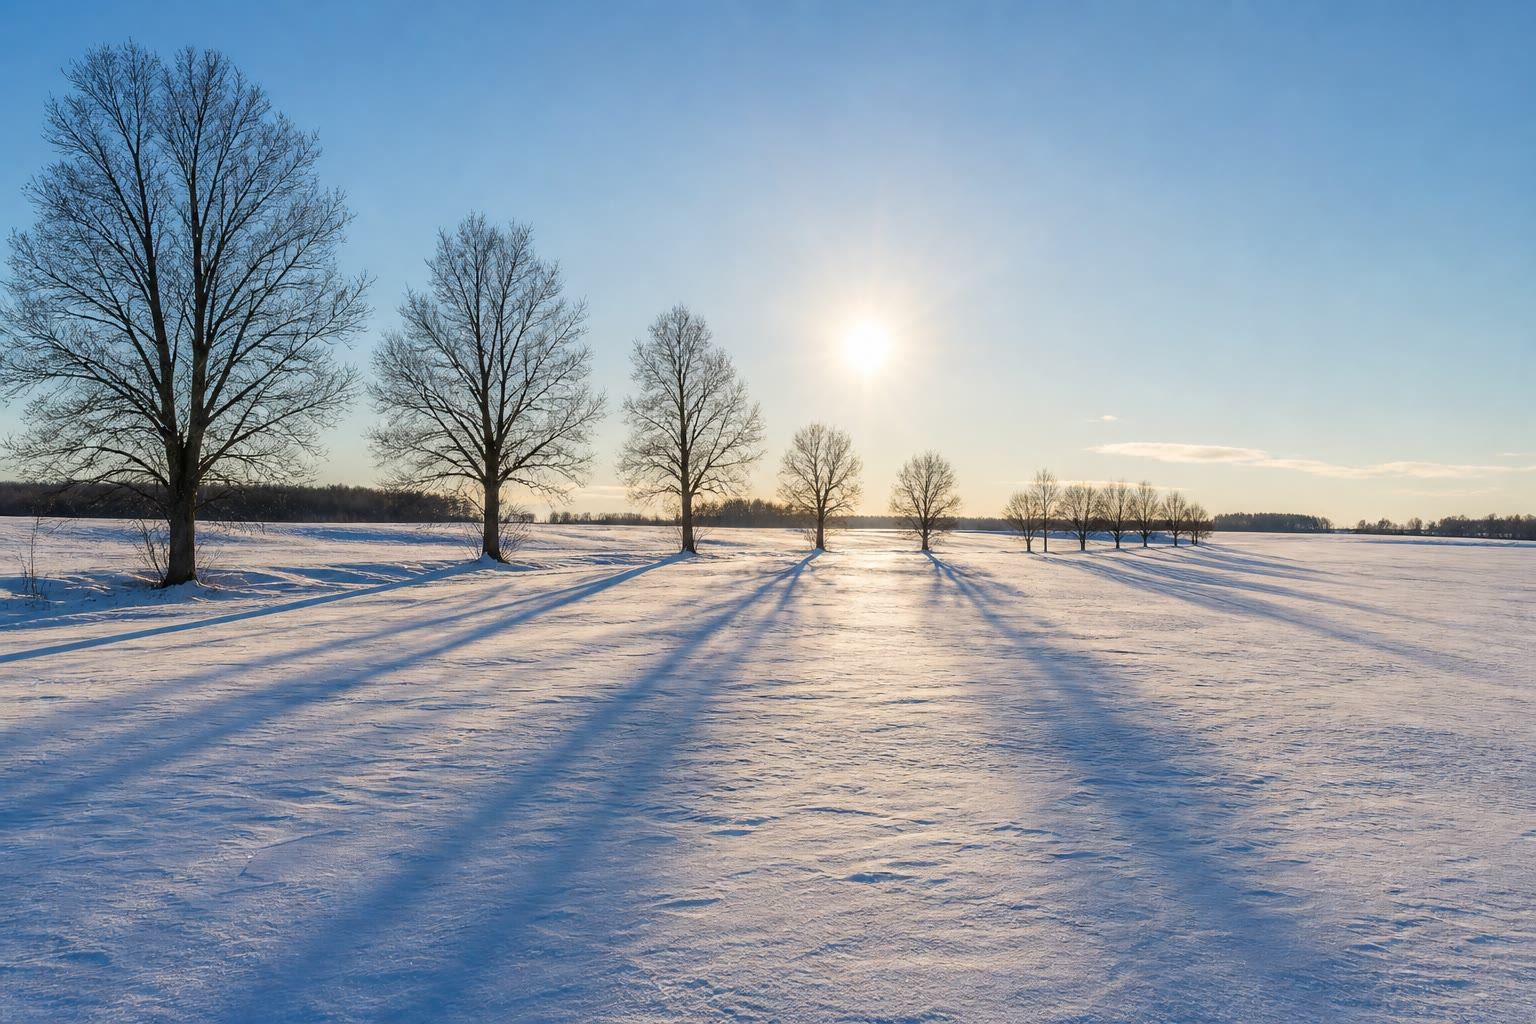
\includegraphics[width=0.58\linewidth]{images/book1/ai/g3-seasons-winter-sun.jpg}

{\small 冬季正午：太阳依然低垂，光线斜射进来，\omterm{def:g1:light-and-shadows:shadow}{影子}在雪地上拉得很长。}
\end{omfigure}

\section{练习}

\begin{exercise}[$\star$]\label{exo:g3:sun-days-seasons:1}
哪个\omterm{def:g3:sun-days-seasons:year}{季节}太阳的运行弧线最高、最长？最低、
最短？这对白天的长短有什么影响？
\end{exercise}

\begin{exercise}[$\star$]\label{exo:g3:sun-days-seasons:2}
一天中什么时刻，立杆的\omterm{def:g1:light-and-shadows:shadow}{影子}最短？正午的\omterm{def:g1:light-and-shadows:shadow}{影子}
日复一日还有什么特别之处？
\end{exercise}

\begin{exercise}[$\star$]\label{exo:g3:sun-days-seasons:3}
同一根立杆在六月的正午\omterm{def:g1:light-and-shadows:shadow}{影子}长为 $2$ 个靴长，
十二月则为 $7$ 个靴长。请借助太阳的
两条“路”解释其中的差异。
\end{exercise}

\begin{exercise}[$\star$]\label{exo:g3:sun-days-seasons:4}
\omterm{def:g3:sun-days-seasons:sundial}{日晷}如何告诉我们时间？它的移动“指针”由什么做成？
\end{exercise}

\begin{exercise}[$\star$]\label{exo:g3:sun-days-seasons:5}
在\cref{met:g3:sun-days-seasons:build}中，为何立杆必须
放在整天有阳光的地方？阴天时，这座钟会
怎样？夜里又会怎样？
\end{exercise}

\begin{exercise}[$\star$]\label{exo:g3:sun-days-seasons:6}
地球绕太阳转一圈要用多长时间？一圈里
包含几个\omterm{def:g3:sun-days-seasons:year}{季节}？从春季开始，把它们按顺序排列。
\end{exercise}

\begin{exercise}[$\star$]\label{exo:g3:sun-days-seasons:7}
一年大约有多少天？还有——来自前一章的问题——
一天有多少\omterm{ex:g2:measuring-time:clock}{小时}？各是地球的哪一种运动造成的？
\end{exercise}

\begin{exercise}[$\star$]\label{exo:g3:sun-days-seasons:8}
请说出两条线索，它们在一周之内从你的窗口
就能看到，借此不用日历即可判断现在是仲夏
还是仲冬。
\end{exercise}

\begin{exercise}[$\star$]\label{exo:g3:sun-days-seasons:9}
你所在的地方是冬季时，地球另一半的孩子们
那里是什么\omterm{def:g3:sun-days-seasons:year}{季节}？这能说明关于“冬天是因为整个地球
离太阳更远”的猜测有什么问题？
\end{exercise}

\begin{exercise}[$\star\star$]\label{exo:g3:sun-days-seasons:10}
一位园丁三月在她的\omterm{def:g1:light-and-shadows:shadow}{影子}钟上摆好了石子。六月时，
\omterm{def:g1:light-and-shadows:shadow}{影子}在标记的时刻不再碰到这些石子。
立杆动了吗？请说明偏移的是什么，并借助
\cref{ex:g3:sun-days-seasons:shadowlength}来解释。
\end{exercise}

\begin{exercise}[$\star\star$]\label{exo:g3:sun-days-seasons:11}
一位探险者醒来时没带手表，也没有手机，看到
太阳恰好在最高处；一\omterm{ex:g2:measuring-time:clock}{小时}后，她发现帐篷的\omterm{def:g1:light-and-shadows:shadow}{影子}
已经比帐篷还高。她醒来时大约是
什么时刻？她更接近仲夏还是仲冬？
请根据正午规律和\omterm{def:g1:light-and-shadows:shadow}{影子}的长度来论证。
\end{exercise}
